\documentclass[11pt]{article}

% packages
\usepackage{physics}
% margin spacing
\usepackage[top=1in, bottom=1in, left=0.5in, right=0.5in]{geometry}
\usepackage{hanging}
\usepackage{amsfonts, amsmath, amssymb, amsthm}
\usepackage{systeme}
\usepackage[none]{hyphenat}
\usepackage{fancyhdr}
\usepackage[nottoc, notlot, notlof]{tocbibind}
\usepackage{graphicx}
\graphicspath{{./images/}}
\usepackage{float}
\usepackage{siunitx}
\usepackage{esint}
\usepackage{cancel}
\usepackage{enumitem}

% permutations (second line is for spacing)
\usepackage{permute}
\renewcommand*\pmtseparator{\,}

% colors
\usepackage{xcolor}
\definecolor{p}{HTML}{FFDDDD}
\definecolor{g}{HTML}{D9FFDF}
\definecolor{y}{HTML}{FFFFCF}
\definecolor{b}{HTML}{D9FFFF}
\definecolor{o}{HTML}{FADECB}
%\definecolor{}{HTML}{}

% \highlight[<color>]{<stuff>}
\newcommand{\highlight}[2][p]{\mathchoice%
  {\colorbox{#1}{$\displaystyle#2$}}%
  {\colorbox{#1}{$\textstyle#2$}}%
  {\colorbox{#1}{$\scriptstyle#2$}}%
  {\colorbox{#1}{$\scriptscriptstyle#2$}}}%

% header/footer formatting
\pagestyle{fancy}
\fancyhead{}
\fancyfoot{}
\fancyhead[L]{MAS6331 Algebra}
\fancyhead[C]{Midterm}
\fancyhead[R]{Sai Sivakumar}
\fancyfoot[R]{\thepage}
\renewcommand{\headrulewidth}{1pt}

% paragraph indentation/spacing
\setlength{\parindent}{0cm}
\setlength{\parskip}{10pt}
\renewcommand{\baselinestretch}{1.25}

% extra commands defined here
\newcommand{\br}[1]{\left(#1\right)}
\newcommand{\sbr}[1]{\left[#1\right]}
\newcommand{\cbr}[1]{\left\{#1\right\}}

\newcommand{\dprime}{\prime\prime}

% bracket notation for inner product
\usepackage{mathtools}

\DeclarePairedDelimiterX{\abr}[1]{\langle}{\rangle}{#1}

\DeclareMathOperator{\Span}{span}
\DeclareMathOperator{\nullity}{nullity}
\DeclareMathOperator\Aut{Aut}
\DeclareMathOperator\Inn{Inn}
\DeclareMathOperator{\Orb}{Orb}
\DeclareMathOperator{\lcm}{lcm}
\DeclareMathOperator{\Hol}{Hol}
\DeclareMathOperator{\Jac}{Jac}
\DeclareMathOperator{\rad}{rad}
\DeclareMathOperator{\Tor}{Tor}
\DeclareMathOperator{\End}{End}
\DeclareMathOperator{\Gal}{Gal}
\DeclareMathOperator{\id}{id}

% set page count index to begin from 1
\setcounter{page}{1}

\begin{document}
\begin{enumerate}
    \item \textit{Proof.}
    \begin{enumerate}
        \item The factorization of $x^m-1$ in $\mathbb{Z}[x]$ is given by \[x^m-1 = \prod_{d\mid m}\Phi_d(x) = \Phi_m(x)\prod_{\substack{d\mid m \\ d\neq m}}\Phi_d(x).\] (as seen in the notes or in Dummit and Foote) Evaluating the above at $x = a$, we have \[a^m-1 = \Phi_m(a)\prod_{\substack{d\mid m \\ d\neq m}}\Phi_d(a);\] by reducing modulo $p$, since $\Phi_m(a)\equiv 0 \mod p$, we have \[a^m-1 = \Phi_m(a)\prod_{\substack{d\mid m \\ d\neq m}}\Phi_d(a)\equiv 0\mod p.\] If $a$ was not relatively prime to $p$, then $p\mid a$ so that $a^m-1\equiv -1$, which by the above cannot happen.
        
        Hence $a$ is relatively prime to $p$; i.e., $a\in \mathbb{F}_p^\times$.
        
        We show the order of $a$ in $\mathbb{F}_p^\times$ is $m$: Certainly the order of $a$ divides $m$ since $a^m-1\equiv 0\mod p$; suppose by contradiction that $a$ had order $j$ dividing $m$ with $j<m$. Then $a^j-1 = \prod_{d\mid j}\Phi_d(a) = 0$, so there is some $d^\prime\mid j$ with $\Phi_{d^\prime}(a) = 0$. But $x^j-1 = \prod_{d\mid j}\Phi_d(x)$ is a factor of $x^m-1 = \prod_{d\mid m}\Phi_d(x)$ since $j\mid m$. Since $d^\prime\neq m$ it follows that $x^m-1$ has a multiple root at $a$ over $\mathbb{F}_p$ ($\Phi_{d^\prime}(a) = \Phi_{m}(a) = 0$). This is in contradiction to the separability of $x^m-1$ over $\mathbb{F}_p$, as $x^m-1$ is coprime with $mx^{m-1}\neq 0$ since $p\nmid m$.
        
        Thus $a$ has order exactly $m$ in $\mathbb{F}_p$.
        \item We show that if $p$ does not divide $m$, then $p\equiv 1 \mod m$. In this case $a$ has order $m$ by part (a). Since $\mathbb{F}_p^\times$ has order $\phi(p) = p-1 $, the order of $a$ divides $p-1$. So $cm+1 = p$ for some integer $c$, from which it follows that $p \equiv 1\mod m$.
        
        Hence $p$ divides $m$ or $p\equiv 1\mod m$.
        \item By prime factorization, there are finitely many primes dividing $m$. Since $f(x) = x^m-1$ is a nonconstant monic polynomial, there are infinitely many (odd) primes which are divisors of at least one of $f(1)$, $f(2)$, $f(3)$, $f(4),\dots$. Only finitely many of these primes could divide $m$, so for the remaining infinitely many primes they must be congruent to $1$ modulo $p$ by part (b).
        
        Hence there are infinitely many primes $p$ such that $p\equiv 1\mod m$. \qed
    \end{enumerate}
    \item \phantom{*}
    \begin{enumerate}
        \item We use the bonus characterization of Galois extensions from the notes: The finite separable extension $K/F$ is Galois if and only if every embedding of $K$ into $L$ fixing $F$ is an automorphism of $K$ fixing $F$ (note every automorphism of $K$ fixing $F$ may be viewed as an embedding). It follows then that $N_{K/F}(\alpha) = \prod_{\sigma\in\Gal(K/F)}\sigma(\alpha)$ since $\Gal(K/F)$ is the group of all automorphisms of $K$ fixing $F$.
        \item Let $G = \Gal(L/F)$ and $H = \Gal(L/K)$. By the Galois correspondence (from notes/Dummit and Foote), the embeddings of $K$ into $L$ fixing $F$ are in bijective correspondence with the cosets $\sigma H$ of $G/H$. So $N_{K/F}(\alpha) = \prod_{\sigma H\in G/H}\sigma(\alpha)$. 
        
        We recall that $G$ acts transitively by multiplication on $G/H$: Given $\sigma H,\tau H$, since $G$ is a group find $\sigma^\prime$ such that $\sigma^\prime \sigma = \tau$ so that $\sigma^\prime(\sigma H) = (\sigma^\prime \sigma)H = \tau H$. Thus $g (G/H)$ is in bijection with $G/H$ (the multiplication permutes the cosets).
        
        Then consider the polynomial $f(x) = \prod_{\sigma H\in G/H}(x-\sigma(\alpha))\in K[x]$. For any element $\tau\in G$ we extend $\tau$ to a map on $K[x]$ by letting $\tau$ be a homomorphism such that $x\mapsto x$. Then $\tau(f(x)) = \prod_{\sigma H\in G/H}(x-(\tau\sigma)(\alpha)) = \prod_{\sigma H\in G/H}(x-\sigma(\alpha))$ since multiplication by $\tau$ simply permutes the cosets $\sigma H$ (and we do not need to worry about which coset representatives we end up with after the multiplication since they differ by a factor in $H$, but $H$ fixes $K$). Since $\tau$ was arbitrary, it follows that $G$ fixes $f(x)$, meaning all of the coefficients of $f(x)$ actually were in $F$. So $f(x)\in F[x]$, and observe that $\prod_{\sigma H\in G/H}\sigma(\alpha)$ is, up to a sign, the constant term of $f(x)$, which is in $F$ as desired.
        \item Each of the embeddings are homomorphisms, so \[N_{K/F}(\alpha\beta) = \prod_\sigma \sigma(\alpha\beta) = \prod_\sigma \sigma(\alpha)\sigma(\beta) = \prod_\sigma \sigma(\alpha)\prod_\sigma \sigma(\beta) = N_{K/F}(\alpha)N_{K/F}(\beta).\]
        \item Since $F(\alpha)$ is a subfield of $K$ containing $F$ and $m_\alpha(x)$ is degree $d$ (so $[F(\alpha)\colon F] = d$), it follows by the tower law that $n = [K\colon F] = [K\colon F(\alpha)][F(\alpha)\colon F] = [K\colon F(\alpha)]d$. Hence $d\mid n$.
        
        Observe that the minimal polynomial $m_\alpha(x)$ divides $\prod_{\sigma H\in G/H}(x-\sigma(\alpha))$ since $\alpha$ is a root of the latter. It follows that there is a product $\prod_{i=1}^d(x-\sigma_i(\alpha))$ of $d$ distinct factors (since $K$ is a separable extension $m_\alpha(x)$ has distinct roots) with $\prod_{i=1}^d(x-\sigma_i(\alpha)) = m_\alpha(x)$, where $\sigma_i$ are coset representatives for $d$ of the cosets in $G/H$ and $\sigma_1 = \id_K$.
        
        Observe further that since $m_\alpha(x)$ is over $F$, that any embedding of $K$ into $L$ fixing $F$ will only permute the factors of the product. Consider a representative $\sigma$ of some coset $\sigma H$ not equal to $\sigma_iH$ for $1\leq i\leq d$. Then the product $\prod_{i=1}^d(x-\sigma\sigma_i(\alpha))$ is equal to $m_\alpha(x)$ but appears as a factor of $\prod_{\sigma H\in G/H}(x-\sigma(\alpha))$ distinct from $\prod_{i=1}^d(x-\sigma_i(\alpha)) = m_\alpha(x)$ (so $m_\alpha(x)$ is a repeated factor in the whole product). We should be able to iterate this process (by finding successive embeddings $\sigma$ such that $\prod_{i=1}^d(x-\sigma\sigma_i(\alpha))$ are distinct from the ones already found) to find $m_\alpha(x)$ as a repeated factor of $\prod_{\sigma H\in G/H}(x-\sigma(\alpha))$ exactly $n/d$ times since $\abs{G/H} = [K\colon F] = n$ by the Galois correspondence.
        
        Then see that with $x= 0$, we have $a_0^{n/d} = m_\alpha(0)^{n/d} = \prod_{\sigma H\in G/H}(-\sigma(\alpha)) = (-1)^nN_{K/F}(\alpha)$. Therefore the $d$ distinct roots of $m_\alpha(x)$ are the $d$ distinct Galois conjugates of $\alpha$ which appear as repeated factors of $N_{K/F}(\alpha)$, and by multiplying the above equality by $(-1)^n$ on both sides obtain $N_{K/F}(\alpha) = (-1)^na_0^{n/d}$.
    \end{enumerate}
    \item Exam questions can be fun.
    \begin{enumerate}
        \item Since norms are multiplicative, if $\alpha$ was a square of an element $\beta$ in $K$ then its norm is necessarily a square of a rational number: $N_{K/\mathbb{Q}}(\alpha) = N_{K/\mathbb{Q}}(\beta^2) = N_{K/\mathbb{Q}}(\beta)^2$, and $N_{K/\mathbb{Q}}(\beta)\in\mathbb{Q}$.
        
        However, using Wolfram Alpha the norm of $\alpha$ is computed to be $277$: The Galois group $G$ of $\mathbb{Q}(\zeta_3,\sqrt[3]{2})/\mathbb{Q}$ (the splitting field of $x^3-2$) is given by $\abr{\sigma,\tau}\cong S_3$ (notations as in Dummit and Foote), where $\sigma$ is the map which fixes $\zeta_3$ and sends $\sqrt[3]{2}$ to $\zeta_3\sqrt[3]{2}$ (order 3), and $\tau$ fixes $\sqrt[3]{2}$ and sends $\zeta_3$ to $\zeta_3^2$ (order 2). The subgroup $\abr{\tau}$ is the fixed field for $\mathbb{Q}(\sqrt[3]{2})$, from which it follows we use the three coset representatives in $G/H$ coming from $\abr{\sigma}$ to compute the norm. \begin{figure}[h]
            \centering
            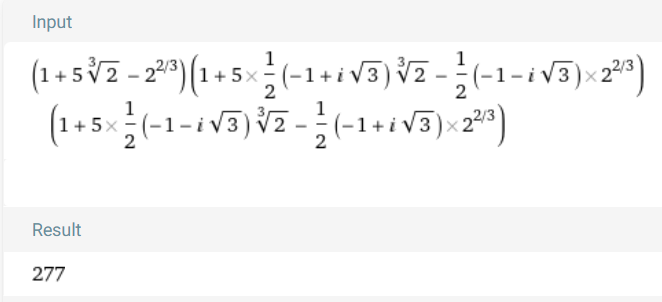
\includegraphics[scale=0.75]{wolfram.PNG}
          \end{figure}
          
        Since $277$ (it is prime as checked by computer) is not a square of a rational number, we cannot have that $\alpha$ is a square of an element in $K$. Hence $x^2-\alpha$ is irreducible over $K$ (it has no roots in $K$).
        \item If $n$ is a sum of two integer squares $x^2+y^2$ then $n$ may be given by the norm of $x+iy\in\mathbb{Q}(i)$, which is $(x+iy)(x-iy) = x^2+y^2$. [$\mathbb{Q}(i)/\mathbb{Q}$ is a quadratic Galois extension and hence only has complex conjugation as a nontrivial element in its Galois group.]
        
        So if $n = N_{\mathbb{Q}(i)/\mathbb{Q}}(x+iy)$ and $m = N_{\mathbb{Q}(i)/\mathbb{Q}}(a+ib)$ for $x,y,a,b\in\mathbb{Z}\subset\mathbb{Q}$, then with the norm being multiplicative we have $nm = N_{\mathbb{Q}(i)/\mathbb{Q}}((x+iy)(a+ib))$. But $(x+iy)(a+ib) = (a x - b y) + i (b x + a y)$ with $ax-by,bx+ay\in\mathbb{Z}$. It follows that $nm$ is also a sum of two integer squares. [I suppose we could have also directly taken the product $nm = (x+iy)(x-iy)(a+ib)(a-ib)$ and shown it is a sum of squares of integers.]
        \item It suffices to produce one such solution; in particular, to produce one element of $\mathbb{Q}(\sqrt{3})$ whose norm is $1$. Observe that the norm of $a+\sqrt{3}b\in\mathbb{Q}(\sqrt{3})$ for $a,b\in\mathbb{Z}\subset \mathbb{Q}$ is $a^2-3b^2$. So $a,b$ satisfy $a^2-3b^2 = 1$ if and only if $a+\sqrt{3}b$ has norm $1$. [$\mathbb{Q}(\sqrt{3})/\mathbb{Q}$ is a quadratic Galois extension with $\sqrt{3}\mapsto-\sqrt{3}$ as the nonidentity element of its Galois group.]
        
        We have that the norm of $2+\sqrt{3}$ is $(2+\sqrt{3})(2-\sqrt{3}) = 4-3 = 1$. Then consider $(2+\sqrt{3})^2 = 7+4\sqrt{3}\in\mathbb{Q}(\sqrt{3})$, which also has norm $1$ since the norm is multiplicative. Iterate this process.
        
        By taking positive integer powers of $2+\sqrt{3}$ one ought to find an infinite family of elements of the form $a+\sqrt{3}b$ with $a,b\in\mathbb{Z}$ whose norm is $1$ (as the norm is multiplicative). When taking powers of $2+\sqrt{3}$ we only obtain integer coefficients for $1$ and $\sqrt{3}$ by the binomial formula or induction. We check that each power is distinct. If $(2+\sqrt{3})^k = (2+\sqrt{3})^j$ with $k>j\geq 1$ then $(2+\sqrt{3})^{k-j} = 1$ which is impossible. [If we want to think about ordering of real numbers, any positive integer power of $2+\sqrt{3}$ is strictly greater than $1$.] Hence $\cbr{(2+\sqrt{3})^k\mid k\in\mathbb{Z}_+}$ is an infinite set of elements of $\mathbb{Z}(\sqrt{3})\subset \mathbb{Q}(\sqrt{3})$ which have norm $1$; equivalently, each element $a+\sqrt{3}b$ in the above set produces a unique pair $a,b$ of integers which satisfy $a^2-3b^2=1$.

        Hence $x^2-3y^2=1$ has infinitely many integer-valued solutions.
    \end{enumerate}
    \item Feedback: I thought this was pretty challenging, and I did not figure out everything. I don't know why the primes in the first problem had to be odd and my first guess is to think that something might go wrong in characteristic $2$. The second question was also definitely harder and I am not sure how to fix the proof for the last part in particular as it is very scuffed. But the third problem didn't seem too bad unless somehow I missed something very big in each part.
    
    I didn't find any of the topics boring but some were certainly more interesting than others: I found the segments on cyclotomic field extensions and Kummer theory pretty neat as well as of course the actual Galois correspondence and the many ways one could use it, but things like dealing with finite fields seemed less interesting to me, perhaps because we did not spend as much time working with them. I don't seem to remember the difficulty varying too much between the topics. 

    I am excited to learn category theory from the perspective of an algebraist, since it would be different from whatever I've seen in my topology classes.
\end{enumerate}
\end{document}